\documentclass{acm_proc_article-sp}
\usepackage{algorithm2e}
\usepackage{float}
\usepackage{qtree}

%%% Header
\title{Facilitating Large-Scale Graph Search Algorithms with Lock-Free Concurrent Pair Heaps}

\numberofauthors{3}

\author{
\alignauthor
Jeremy Mayeres \\
\email{jeremym@knights.ucf.edu}
%
\alignauthor
Charles Newton \\
\email{newton@knights.ucf.edu}
%
\alignauthor
Peter Tonner \\
\email{ptonner@knights.ucf.edu}
}
%%%

\begin{document}
\maketitle
\begin{abstract}
This paper introduces a lock-free version of a Pairing heap.
Dijkstra's algorithm is a search algorithm to solve
the single-source shortest path problem. The efficiency
of Dijkstra's algorithm is asymptoticly improved
from $\mathcal{O}(|V|^2)$ to $\mathcal{O}(|E| + |V|\log(|V|))$ when
an operation is available to decrease the recorded distance of a vertex
to the target source in constant time (\texttt{decreaseKey}.)
The performance of Dijkstra's algorithm
also improves when threads can also perform work concurrently (in particular, when
\texttt{decreaseKey} calls occur concurrently.) However, current implementations of
\texttt{decreaseKey} on popular backing data structures such as Pairing heaps and Fibonacci heaps
severely limit concurrency. Lock-free techniques can improve the concurrency of search structures
such as heaps. In this paper we introduce \texttt{decreaseKey} and \texttt{insert}
operators for Pairing heaps that provide lock-free guarantees while still running in constant time.
We compare our work against a novel \texttt{decreaseKey} operator on Skiplists.
Techniques for parallelizing Dijkstra's algorithm are additionally discussed.

%This project will cover the design and application of lock-free concurrent pairing heaps. Pairing heaps have comparable efficiency to fibonacci heaps, with an easier implementation. A lock-free model of this data structure will be built in Java or C++. As pairing heaps are efficient for graph algorithns, efficiency of the concurrent lock-free pairing heap will be tested using shortest path calculation from Dijkstra's algorithm on large networks.

%We will
%adapt Fredman and Tarjan's pairing heap
%\cite{fredman86} to Shavit and Lotan's
%\cite{shavit00} SkipQueues. Specifically, we
%propose developing an efficient \texttt{decreaseKey}
%operator for SkipQueues.
\end{abstract}

\category{D.1.3}{Concurrent Programming}{Programming Techniques}
\category{E.1}{Lists, stacks, and queues}{Data Structures}
\category{E.1}{Trees}{Data Structures}

\terms{Performance, Algorithms, Parallel Algorithms}

\keywords{Lock-free data structures, Pairing heap, Heap, Skiplist, Skip queue, Lock-free heap, Lock-free Pairing heap} 

\section{Overview of Progress}
This section gives a short overview of the current
state of our class project. We have developed two
lock-free operators on Pairing Heaps: \texttt{decreaseKey}
and \texttt{insert}. Although the remaining Pairing Heap functions
do not support concurrency, our lock-free Pairing heap is complete
enough to support a parallelization of Dijkstra's algorithm
without compromising the constant-time performance of the 
\texttt{decreaseKey}
operation (which allows Dijkstra's algorithm to run
in $\mathcal{O}(|E| + |V|\log(|V|))$ time.)
We have additionally created an optimization for Skiplists that,
in some circumstances, allow calls to \texttt{decreaseKey} to
execute faster than successive \texttt{delete} and \texttt{insert}
calls.

\section{Introduction}
Dijkstra's algorithm \cite{dijkstra59} is a search
algorithm that solves the (single-source) shortest
path problem for directed graphs with non-negative
weights. It has wide applications in Internet routing
(see, e.g., the shortest-path calculation in the OSPF
routing protocol \cite{rfc5340}) and other scheduling
algorithms that depend on finding optimal paths.

Using a naive data structure (such as a standard binary heap)
results in Dijkstra's algorithm having runtime of $\mathcal{O}(|V|^2)$, where $|V|$
is the number of vertices in the graph. Fredman and Tarjan have
introduced \cite{fredman87} a heap variant, called the Fibonacci heap,
where the \texttt{decreaseKey} operation takes $\mathcal{O}(1)$ time
(amortized.) This allows Dijkstra's algorithm to run in $\mathcal{O}(|E| + |V|\log(|V|))$
time, where $|E|$ is the number of edges in the graph.
However, in practice, Fibonacci heap have large constants that
cause it to be slower than standard heap-backed priority queues
on many practical graphs.

%\begin{figure}[H]
\begin{algorithm}[h]
  %\SetLine
  \SetKwFunction{deleteMin}{deleteMin}
  \SetKwFunction{decreaseKey}{decreaseKey}
  \KwIn{A weighted graph $G=(V,E,W)$ and target node $x$}
  \KwOut{The shortest distance from $x$ to every vertex $v \in V$}
  \Begin{
    \ForEach{$v \in V$}{
      $v$.priority $\leftarrow$ $\infty$\;
      $v$.previous $\leftarrow$ NULL\;
    }
    $x$.priority = 0\;
    $PQ$.insert($x$)\;
    \While{!$PQ$.empty}{
      $u$ $\leftarrow$ \deleteMin{$PQ$}\;
      \ForEach{$v$ where $(v,u) \in E$}{
        $newDist$ $\leftarrow$ $u$.priority + weight($v$,$u$)\;
        \If{$newDist < v$.priority}{
          $oldDist$ $\leftarrow$ $v$.priority\; 
          $v$.priority $\leftarrow$ $newDist$\;
          $v$.previous $\leftarrow$ $u$\;
          \decreaseKey($oldDist - newDist$, $v$, $PQ$)\;
        }
      }
    }
  }
\caption{Dijkstra's algorithm. The main loop comprises a critical section which presents difficulties when parallelizing.}
\label{alg:dijk}
\end{algorithm}
%\end{figure}

This deficiency led Fredman and Tarjan to develop the Pairing heap \cite{fredman86}, which
is simpler than Fibonacci heaps and has better performance in practice. Precise run-time bounds are, unfortunately, currently unknown. 
Pettie \cite{pettie05} has shown the \texttt{decreaseKey} operation takes between $\Omega(\log \log n)$ and $\mathcal{O}(2^{2\sqrt{\log\log n}})$ (amortized) time based on previous work by Fredman \cite{fredman99}.

Current attempts
to parallelize Dijkstra's algorithm rely on \texttt{decreaseKey} operations that have worse asymptotic performance
than Pairing heaps provide. For example, to back Dijkstra's algorithm with Shavit and Lotan's
concurrent priority queue \cite{shavit00} requires the user implement \texttt{decreaseKey} by deleting 
the target from the heap and reinserting it with a decreased value. Both of these operations occur run in
$\mathcal{O}(\log n)$.

To our knowledge, there have been no attempts to construct highly concurrent Heap data structures
with lock-free guarantees that have an efficient \texttt{decreaseKey} implementation.
In this paper we introduce a lock-free variant of the Pairing heap
that allows the \texttt{decreaseKey} and \texttt{removeMin} operations
to be executed in parallel
without the use of locks. Our lock-free \texttt{decreaseKey} operation has an asymptotic time complexity
equal to Fredman and Tarjan's original \texttt{decreaseKey} implementation.

\section{Related Work}
Currently, the most common way to implement Dijkstra's algorithm in
a parallel manner is to partition the graph and apply
Dijkstra's algorithm on
each subgraph \cite{crauser98}. In this section we outline
some of the novel approaches to constructing concurrent priority queues
previously found in the literature.

\subsection{Non-Lock-Free Parallel Heaps}

Nageshwara et al. \cite{nageshwara88} have implemented a priority queue heap with concurrent insert and delete operations. These operations are not lock-free but represent an attempt in the literature to create a concurrent heap model. Their model only scales to $\log(n)$ processors accessing a heap of $n$ nodes. The binary heap implementation presented in their paper modifies the insert operation to work from top to bottom, rather than bottom up. This ensures that inserts can be run without deadlocks with concurrent delete operations, which also run top to bottom. While pairing heaps do not require the same method for inserting and deleting, this style of operation design, where different operations are forced to traverse the tree in the same direction, may be useful in the lock-free pairing heap solution.

Driscoll et. al \cite{driscoll88} have introduced a variant of Fibonacci heaps, called
relaxed heaps, that allows for easier parallelization. However, their approach
is complicated \cite{elmasry10} and, in practice, performs worse than Fibonacci heaps \cite{moret94}.  

\subsection{Automatically Generated Lock-Free Heaps}

In this section we consider how some approaches that automatically
transform sequential data structures into lock-free, concurrent data
structures could be applied to concurrent pairing heaps.

Herlihy \cite{herlihy93} has introduced a universal method of automatically
transforming sequential objects
into concurrent, lock-free objects with very few assumptions about the behavior
of the sequential object. In his method, all threads share a pointer to
the sequential object and a version / timestamp of the object.
When a concurrent operation is called, the object is copied into
a new location in memory and operated upon with a corresponding sequential operation.
The shared pointer is updated if the current timestamp matches the timestamp noted at the beginning
of execution. Otherwise,
the operation is repeated with a new copy of the object. This could lead to the construction
of a lock-free pairing heap that copies itself into memory, performs the related sequential
operation, and updates the state of the object to reflect these modifications (assuming no
other thread has made changes.) However, as Herlihy notes, this automatic transformation
is only suitable for objects which can be efficiently copied (i.e., ``small objects.'')
This would not be appropriate for our particular use-case since we are considering
very large heaps.

Anderson and Moir \cite{anderson99} have improved on Herlihy's approach by
automatically keeping track of locations in memory a sequential operation
reads from and writes to. Only modified blocks of memory are copied. Hence,
this solves some issues with performance when only small portions of a data
structure are modified. For example, consider updating the head of a linked-list backed queue.
With Herlihy's technique, the entire list would need to be copied, but the modification
to the data structure only involves updating the head pointer.
However, this method handles contention poorly if many operations
access the same blocks of memory (as is the case with the \texttt{deleteMin}
operation of a heap.)

\subsection{Concurrent Priority Queues and Heaps}
Shavit and Lotan have constructed \cite{shavit00}
a concurrent priority queue, called a SkipQueue,
based on Pugh's SkipList
\cite{pugh90} data structure.
Sundell and Tsigas \cite{sundell05} have improved on Shavit's
and Lotan's method to create a fully lock-free concurrent
priority queue.

Hunt et al. \cite{hunt96} have introduced an array-backed priority
queue with very fine-grained locks. Their approach
builds on previous work by Rao and Kumar
\cite{rao88} that showed contention on heaps can be greatly decreased
by having the \texttt{deleteMin} and \texttt{insert} operations proceed in
the same (top-down) directions. (If the operations proceed in opposite directions,
this opens a possibility for deadlocks.) However, this increases the
time complexity
of an \texttt{insert} operation to $\mathcal{O}(\log n)$.
The main contribution of Hun et al.'s
approach is that $\mathcal{O}(1)$ performance on a bottom-up \texttt{insert}
can be
preserved without introducing the possibility for deadlocks
by 1) ordering the acquisition of locks, 2) applying
tags / timestamps to avoid the ABA problem, and 3) avoiding overlap
of search paths.

Israeli and Rappoport have developed \cite{israeli93} a wait-free
concurrent heap. However, their implementation uses atomic operations
that are not widely available in today's hardware.

\subsection{Concurrent Fibonacci and Skew Heaps}
Jones \cite{jones89} has constructed a concurrent Skew heap that uses fine-grained
locks (as opposed to locking the entire heap structure) to allow parallel \texttt{insert} and \texttt{deleteMin} operations
without violating the heap invariant. In a Skew heap, each node has three pointers:
two children pointers and one sibling pointer that points to the next node at the same
depth. Jones defines a bubble as the set of all pointers a Skew heap
operation will read or modify before completing its task. An operation must
acquire all the locks in its bubble before performing any modifications. This
granular lock structure allows disjoint heap operations to complete concurrently.

Huang and Weihl \cite{huang91} have constructed a concurrent Fibonacci heap
that allows threads to concurrently perform \texttt{insert}, \texttt{decreaseKey}, and
\texttt{deleteMin} operations. The data structure is backed by a circular doubly-linked
list. An issue with Huang and Weihl's approach is that \texttt{deleteMin} is not
linearizable: threads may access the minimum element of the Fibonacci heap out of
order, (i.e., \texttt{deleteMin} does not necessarily return the minimum element in the heap at
the point in time it is called), although the element is guaranteed to be reasonably small (``promising'') compared to the other
elements in the heap. However, this presents problems with Dijkstra's algorithm and other
graph algorithms that require a strict definition of \texttt{deleteMin}.

\subsection{Other Highly Concurrent Attempts}
Michael and Scott's \cite{michael96} lock-free FIFO queue allows enqueue
and dequeue operations to proceed concurrently on a
single link-list backed queue. Moir et al. have developed
\cite{moir05} a variant of the Michael-Scott queue that applies
an elimination back-off technique to eliminate contention for the
head / tail regions of the linked list. Previously, this
technique was used by Shavit and Touitou \cite{shavit97} to create
concurrent counters and Hendler et al.  \cite{hendler04} to create concurrent LIFO
stacks. Moir's technique is a natural generalization of the elimination
approach used in LIFO stacks: have the backed-off enqueue operations
eliminate against a backed-off dequeue operation once all the elements prior
to the back-off point have been dequeued.

\section{Skiplists}
Skiplists were introduced by William Pugh \cite{pugh90} as a way
to avoid expensive rebalancing in tree structures while
still retaining desirable properties of balanced
trees such as $\mathbb{O}(\log n)$ search. The basic
idea behind Skiplists is to allow the tree structure
to be controlled by a pseudorandom number generator (PRNG). Thus,
a Skiplist only gives probabilistic guarantees that it will
produce a balanced tree structure.
However, pathologically bad structures that cause the data structure to degrade
to a search complexity of $\mathbb{O}(n)$ are very unlikely. Also, since Skiplists
do not rebalance themselves, input keys are typically uniformly mapped into another
set (e.g., by using a hash function) to avoid pathological inputs.

A Skiplist is a set of linked lists with ordered elements.
Each linked list is assigned a level $0 \leq i \leq M$ which describes
the density of the linked list at that level. The first
level (level 0) contains all the elements in the Skiplist.  We
adopt the notation that $L(i)$ denotes the list at level
$i$. $L(0)$ (the bottom-most level) is guaranteed to 
contain all the elements inside the Skiplist. For each higher level
$i > 0$, $L(i)$
is expected to contain $\frac{1}{2}|L(i-1)|$ elements.
In Fig. \ref{fig:skiplist}, a Skiplist containing
$L(0) = \{1,3,9,11,15\}$ is presented.

\begin{figure}[H]
  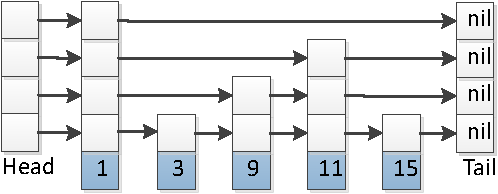
\includegraphics[width=0.5\textwidth]{img/skiplist-crop.pdf}
  \caption{A Skiplist representation of $\bf \{1,3,9,11,15\}$. The levels of
each node, respectively, are 3, 0, 1, 2, and 0.}
  \label{fig:skiplist}
\end{figure}

\subsection{Core Operations}

We now outline a few operations on Skiplists. In general, these are
quite similar to their linked-list counterparts. In fact, each Skiplist
operation can be decomposed into a sequence of linked-list operations that
each affect
one level of the Skiplist.

Suppose we want to search for element $e$. First,
we look at the list at $L(M)$ and traverse it linearly until we encounter
an element greater or equal to $e$.  If we encounter $e$, then we stop.
If we found an element greater than $e$, we repeat this procedure from
this new starting point. If we only encountered the tail of the list, then we
repeat the procedure starting from the first element in $L(M-1)$. This procedure
repeats until we successfully locate $e$. If we encounter either an element
greater than $e$ or end of the list at $L(0)$ we conclude $e$ is
not contained in the Skiplist. See Figs. \ref{fig:skiplist:search3} and \ref{fig:skiplist:search15}
for sample search runs on the Skiplist presented in Fig. \ref{fig:skiplist}.

To insert an element $e$ into a Skiplist, we first perform a search for the element
as previously described. However, we also keep track of additional information.
The insertion point is determined by where we stop searching at $L(0)$. Throughout the
search process, an array
$\texttt{previous}[i]$ is maintained that contains all the right-most pointers (at level $i$)
to elements left of the insertion point. An array $\texttt{next}[i]$ is given the previous values
of each pointer in $\texttt{previous}[i]$. To insert $e$, we assign it a random level $l$, set 
all the right-most pointers in $\texttt{previous}[i]$ for $0 \leq i \leq l$ to $e$ and set
the pointers emanating from $e$ to $\texttt{next}[i]$ for $0 \leq i \leq l$. Insertion has
the visual effect of simply splicing $e$ into the Skiplist (see Fig. \ref{fig:skiplist:insert5}.)

To delete an element $e$ from a Skiplist, we first search for the element (as we did for insertion).
If the element is not found, we are done. Otherwise, we should map each pointer in $\texttt{previous}[i]$
to the value in $\texttt{next}[i]$ for $0 \leq i \leq l$, where $l$ is the level of $e$. See Fig. \ref{fig:skiplist:insert5} for an illustration of deleting an element from a Skiplist.

\subsection{Additional Operations}
Pugh has defined \cite{pugh90a} a number of useful
operations such as merging Skiplists, splitting Skiplists, and
concatenating two Skiplists together when all the keys in one Skiplist
are less than or equal to the smallest key in a second Skiplist. However,
an operation that decreases the value of an element in a Skiplist (besides
simply deleting the old value and reinserting the decreased value) was not present and
we were unable to find a description of this operation in the literature.

\begin{figure}[H]
  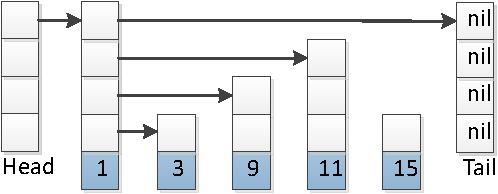
\includegraphics[width=0.5\textwidth]{img/skiplistSearch-crop.pdf}
  \caption{Skiplist traversal for finding the element 3 in the Skiplist presented in Fig. \ref{fig:skiplist}}
  \label{fig:skiplist:search3}
\end{figure}

\begin{figure}[H]
  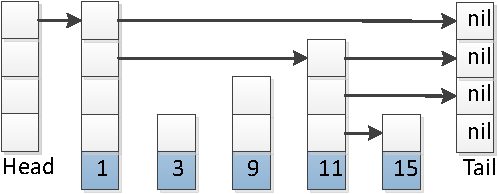
\includegraphics[width=0.5\textwidth]{img/skiplistSearch15-crop.pdf}
  \caption{Skiplist traversal for finding the element 15 in the Skiplist presented in Fig. \ref{fig:skiplist}}
  \label{fig:skiplist:search15}
\end{figure}

\begin{figure}[H]
  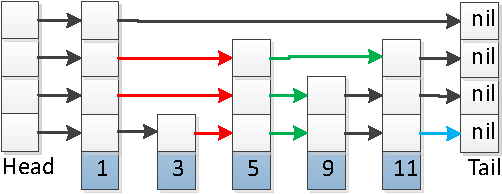
\includegraphics[width=0.5\textwidth]{img/skiplistInsert5-crop.pdf}
  \caption{Illustration of insertion and removal. 5 has been inserted into the Skiplist. Red indicates pointers contained in $\texttt{previous}[i]$, and green indicates pointers contained in $\texttt{next}[i]$. 15 has also been removed from the Skiplist and updated pointers for this operation are in blue.}
  \label{fig:skiplist:insert5}
\end{figure}

\subsection{Lock-Free Skiplists}
Shavit and Lotan's Skipqueue \cite{shavit00} is a modification
of Pugh's Skiplist that gives its operations lock-free guarantees.
We present a high-level technical summary of their work as in
section \textbf{XYZ} we will
build a \texttt{decreaseKey} operator for Skiplists using their approach.
Following with our analogy of Skiplist
operations being composed of operations on the linked lists formed at each level
of the Skiplist, we see that lock-free
operations on Skiplists can be composed of operations on lock-free linked lists.

One subtle issue with Shavit and Lotan's modifications is that $L(i)$ is not necessarily a subset
of all $L(k)$ (for $k < l$): a value's membership is determined by it being
in the lowest level of the Skiplist.
In particular, this means that even if we encounter
a target value in a higher level of the Skiplist, we still must verify it is
linked to the structure in $L(0)$. 

The search, add, and delete operations of a lock-free Skiplist follow the same form as
those we defined on Pugh's Skiplist.
However, here we need to handle the possibility of threads
concurrently modifying the Skiplist. To detect concurrent operations, we
modify our linked list's node datatype from the 2-tuple (\texttt{value}, \texttt{nextPtr[]}) to
the 3-tuple $(\texttt{value}, \allowbreak \langle \texttt{bool}, \allowbreak \texttt{nextPtr} \rangle\texttt{[]}$),
where \texttt{nextPtr} is the datatype used for pointers, and $\langle \texttt{bool}, \allowbreak \texttt{nextPtr} \rangle$
are written / read in a single atomic operation. In Java, this can be implemented
with the \texttt{AtomicMarkableReference} class.
In C/C++, this can be easily implemented by stealing a bit from a word-aligned pointer.
The boolean value serves as a deletion bit that is set whenever a node is removed
from the Skiplist but has yet to be physically removed from the linked list structure. This is
important for avoiding certain interleavings of operations. Consider two threads concurrently accessing
a Skiplist. The first thread reads the deletion mark on an element $a$ at level $i$, and is
interrupted by a second thread which marks the element as deleted. When the first thread resumes,
it will still assume that $a$ is not marked and, if inserting a new element,
could create an untraversable section of the
Skiplist by building on $a$'s next pointer.

To search for an element in a lock-free Skiplist we take the same approach as before, but
we additionally remove any marked nodes from the linked list structure and we always traverse
down to $L(0)$ in order to verify membership. To add an element
into the lock-free Skiplist we construct the \texttt{previous[i]} and \texttt{next[i]} sets
as before and set the next pointers of the new node to \texttt{next[i]}. We also update the
pointers in \texttt{previous[i]} to point to our new node (from level $0$ to level $l$).
If we are unsuccessful at having \texttt{previous[0]} point to our new node, we restart the
whole procedure since either a new node was inserted and the ordering of $L(0)$ may be violated
if we insert or the node at \texttt{previous[0]} was marked for removal.
Note that the linearization point of an add occurs when the element is inserted
into $L(0)$. Once \texttt{previous[0]} is updated, we attempt to update
\texttt{previous[i]} to \texttt{next[i]} in a CAS loop. To handle concurrent changes
during this process (e.g., \texttt{previous[i]} being marked), we recompute the \texttt{previous}
and \texttt{next} arrays whenever an atomic update fails.

Removing an element from a lock-Free Skiplist is analogous to adding an element.
First, we search for the target element and compute our \texttt{previous[i]} and \texttt{next[i]}
arrays. Next, we mark each
\texttt{next} pointer of the target element in a top-down fashion within a CAS loop. When a CAS fails,
we re-read the relevant \texttt{next[i]} as another thread could have modified it (e.g., a
new node was linked to the node we're currently deleting.) When the \texttt{next}
pointer has been marked in $L(0)$, we consider the element removed (this is our linearization
point.) There is no need update any pointers on a removal since subsequent searches will perform
this for us.

\subsection{A decreaseKey operator for Skipqueues}
Keeping track of the \texttt{next[i]} and \texttt{previous[i]}
``windows'' of an element in a Skipqueue leads to a natural implementation
of a \texttt{decreaseKey} operator. Suppose we have located the target element in the
Skipqueue and it has a level of $M$. Let $i^*$ denote the index of the largest value
in the \texttt{next} array that is smaller than the new value of the target. We can use
$\mathtt{next[i}^*\mathtt{]}$ as the starting location for determining a new location
for the decreased value of our target (since every node after $\mathtt{next[i}^*\mathtt{]}$
is greater than our new value.) Aside from the head of the list, the insert is performed
the same as before. If the attempt to insert needs to be restarted, we restart as non-optimized insertion.

The level of the decreased element is bounded above by $M$. On the first (the optimized) insertion attempt we
set the level of the decreased element equal to $M$. This avoids introducing bias into the Skipqueue structure: if we sampled
the new height from the discrete uniform distribution $U(0, M)$ we would force elements to gradually
loose levels. If the optimized insertion attempt fails, there is no restriction placed on the level of the element.

\section{Pairing Heaps}
Pairing heaps were developed by Fredman et al. \cite{fredman86} as
a simpler alternative to Fibonacci heaps that, at least empirically,
do not sacrifice performance.
Pairing heaps are a popular backing data structure
for Dijkstra's algorithm due to its efficient implementation
of the \texttt{decreaseKey} operation. 

% http://www.cise.ufl.edu/~sahni/dsaaj/enrich/c13/pairing.htm is good!

\subsection{Operations on Pairing Heaps}

We provide a sketch of the salient features of pairing heaps.
The main operator defined on pairing heaps is \texttt{meld}, which
accepts two heaps and uses a compare-and-link approach to join
its inputs together. See Fig. \ref{fig:meld} for an example of
melding two heaps together. The roots are compared and the root with the
largest value (assuming we have min-heaps) is added as the left-most
child of the smaller root. Insertion of a node is performed
by constructing a trivial heap containing only the relevant node
and melding it the main heap.

The supported pairing heap operations are as follows:
\begin{itemize}\addtolength{\itemsep}{-1\baselineskip}
\item[] $\mathtt{makeHeap}(h)$\\
\item[] $\mathtt{findMin}(h)$\\
\item[] $\mathtt{insert}(x, h)$\\
\item[] $\mathtt{deleteMin}(h)$\\
\item[] $\mathtt{meld}(h, h')$\\
\item[] $\mathtt{decreaseKey}(\Delta,x,h)$\\
\item[] $\mathtt{delete}(x,h)$\\
\end{itemize}
where $h,h'$ are pairing heaps, $x$ is a target node (or, equivalently,
a target value), and $\Delta > 0$ is the value by which the
target node should be decremented.

\begin{figure}
  \Tree [.3 [.5 \qroof{T_1}.10 [.12 \qroof{T_2}.19 \qroof{T_3}.20 ] \qroof{T_4}.34 ] !{\qframesubtree} [.25 [.19 \qroof{T_5}.20 \qroof{T_6}.21 ] \qroof{T_7}.42 ] ]
  \caption{Melding two min-heaps together (one with root 3 and the other with root 5) with the \texttt{meld} operator. The heap rooted at 5 becomes a subheap of the heap rooted at 3.}
  \label{fig:meld}
\end{figure}

\texttt{deleteMin} removes the minimum (root) element of a pairing heap $H$. Say once the root of the tree is removed we have $n$ sub-trees $H_1, H_2, \dots, H_n$, each with their own individual roots.
For each tuple in the set $\{(H_1, H_2), (H_3, H_4), \dots, \allowbreak (H_{n-1}, H_n)\}$, we meld the two heaps together to form $\{H'_1, \dots, \allowbreak H'_m\}$. It is worth mentioning that this pattern of
grouping into tuples (pairs) is where pairing heaps derive their namesake.
If $n$ is odd, $H_n=H'_m$ is not melded.
Finally, we perform a right-iteration
(similar to foldr) of \texttt{meld} over these $m=\frac{n}{2}$ (or $m=\frac{n-1}{2} + 1$) heaps to construct a newly rebalanced pairing heap $H'$:
\begin{equation*}
  H' = \mathtt{meld}(H'_1, \mathtt{meld}(H'_2, \dots \mathtt{meld}(H'_{m-1}, H'_m) \dots ))
\end{equation*}
To make the ordering $H_1, H_2, \dots, H_n$ unambiguous, we say that $i^\mathrm{th}$ child of $H$ (i.e., the root of $H_i$) is the most recently melded node to the root.
Note here that \texttt{deleteMin} rebalances the tree structure of the pairing heap. See Fig. \ref{fig:deletemin} for an illustration of calling
\texttt{deleteMin} on a Pairing heap.

\begin{figure}
  \begin{enumerate}
   \item[(a)] \Tree [.7 [20 15 8 9 42 ] ] 
   \item[(b)] \Tree [20 15 8 9 42 ]
   \item[(c)] \Tree [.15 20 ]
              \Tree [.8 9 ]
              \Tree [.42 ]
   \item[(d)] \Tree [.15 20 ]
              \Tree [.8 42 9 ]
   \item[(e)] \Tree [.8 [.15 20 ] 42 9 ]
  \end{enumerate}
  \caption{Calling \texttt{deleteMin} on a Pairing heap (a). The root is removed (b) and the children are melded in pairs (c), and then the pairs themselves are melded in right-to-left order (d-e). Note that the resulting heap (e) is more balanced than (a).}
  \label{fig:deletemin}
\end{figure}

\texttt{decreaseKey} is implemented as follows. Suppose
a node $x$ has its value decreased and this new value
violates the heap invariant (i.e., $x$ is now
smaller than its parent.) The subtree rooted
at $x$ is removed from the tree and melded
to the parent tree as previously described.

$\mathtt{delete}(x,h)$ is implemented by delinking the sub-tree $S$ rooted at $x$ from $h$, calling $\mathtt{deleteMin}$ on $S$, and melding the resultant
tree back to $h$.

%\texttt{removeRoot} is implemented in a novel way.
%First, a left-to-right pass is performed
%over the root's children. The children
%are grouped into pairs (this is where
%pairing heaps derive their namesake)
%and the largest child of each pair
%is made a child of the smallest. Next,
%a right-to-left pass is performed over
%the grouped trees and they are merged
%together.

\section{Parallelizing Dijkstra's Algorithm}
\label{sec:dijkstra}
We now consider some issues pertinent to parallelizing a heap-backed
implementation of Dijkstra's algorithm. If \\ \texttt{deleteMin} does not
remove and return the unvisited node in the graph with the smallest distance
from the source node, Dijkstra's algorithm is not guaranteed to solve the shortest-path problem.
A na\"{i}ve approach to running Dijkstra's algorithm in parallel would be to let calls
to \texttt{deleteMin} and \texttt{decreaseKey} haphazardly interleave. However,
the minimum of the heap will change on some call to \texttt{decreaseKey} if
a new value of a node is less than the current value. Thus, some comparison
is needed to see if calls to \texttt{decreaseKey} will produce a new minimum
value in the heap. There are three basic approaches to solving this problem:

\begin{enumerate}
  \item Optimistically continue removing minimum elements from the heap. 
  \item Pessimistically check if any of the new distances are less than the minimum of the heap, and continue
    if the minimum will remain unchanged. This has an advantage over the next method where the decision to continue
    can be made without any modifications to the heap.
  \item Pessimistically assume that \texttt{decreaseKey} will always produce a new minimum and ensure that
    all calls to \texttt{decreaseKey} complete before the next iteration's call to \texttt{deleteMin} executes.
\end{enumerate}

Solution 1 requires complicated interactions between concurrent states of the heap
or requires independent copies of the heap to be made and later merged. Since there are
two choices for every iteration of Dijkstra's algorithm (either the heap's minimum changes
or does not change), a copying approach requires $\mathcal{O}(2^n)$ copies to be made, which is
intractable for large graphs.

Solutions 2 and 3 are both practical. We opt for solution 3 since it is simpler, but
for future work we may consider solution 2.

\section{Lock-Free Pairing Heaps}
In this section we develop lock-free \texttt{insert} and \texttt{decreaseKey}
operators for Fredman et al.'s pairing heap. Our
work relies on the observation that
the specifics of
Dijkstra's Algorithm allow us to make assumptions about how
pairing heap operations interleave. 
We first list some assumptions that we have made about overlapping
calls to operations on the heap. Then, we give a high-level overview
of our lock-free approach before delving into the details of our
\texttt{insert} and \texttt{decreaseKey} operators.
%The second is that both \texttt{insert} and
%\texttt{decreaseKey} can be simplified to create an obvious linearization 
%point without ruining their asymptotic
%$\mathcal{O}(1)$ performance (although at a cost of more work per \texttt{decreaseKey} call.)
%We first list our simplifications and then outline our lock-free approach.

In section \ref{sec:dijkstra} we analyzed the specific performance bottle-necks and other
issues with running Dijkstra's algorithm in parallel. In particular, we noted that the
linearization guarantees provided by presently available lock-free heaps are insufficient for
blindly executing
concurrent calls to \texttt{deleteMin} and \texttt{decreaseKey}. Hence, we assume
these calls will never interleave, and, further, that only concurrent calls to 
\texttt{decreaseKey} overlap.

%(Some language that was either nonsense or unclear, so I'm rewording it.)
%Another issue to discuss involves the role of the parent pointer in a
%Pairing heap's nodes.
%We also make the following simplification to remove \texttt{decreaseKey}
%Recall that, for Pairing Heaps,
%\texttt{delete} was implemented by removing the target node from its parent.
%However,
%Dijkstra's algorithm does not make use of a call to \texttt{delete} and the
%only other reference to node's parent is in \texttt{decreaseKey}'s check if
%the newly decreased value violates the heap invariant. This is
%only an optimization and if this check is removed
%\texttt{decreaseKey} will still run in $\mathcal{O}(1)$ time
%as \texttt{meld} runs in constant time.
%Note the similarities between this less optimized version of
%\texttt{decreaseKey} and \texttt{insert}: both simply meld
%a key to the root of the tree. Additionally, if we assume that
%edges between nodes are unique (i.e., the set of edges is not
%a multiset), then each call to \texttt{decreaseKey} operates
%on a unique key per iteration of Dijkstra's algorithm. This gives
%the useful property that while in the \texttt{decreaseKey}-loop, only
%one thread attempts to read or write a given node's parent field.
%As this does not lead to contention,
%we take no special care at guarding concurrent reads and writes in this case.

%We use a CAS loop to insert a new node (or a newly decreased node)
%at the root (or as a root's child.) Before a node is inserted, the current root and its timestamp
%are recorded. A call to \texttt{meld} makes stateful changes to the heaps in its arguments,
%so we create a copy of the recorded root (this way if CAS is unsuccessful, we haven't
%made any changes to the main heap.) After \texttt{meld} runs, we attempt to CAS our new root
%into place. If CAS fails, we undo the inclusion of the larger node as a child of the smaller node and retry.
%Otherwise, the new node is accessible in the heap.
%This yields a clear linearization point for
%\texttt{decreaseKey} and \texttt{insert}: a node is considered successfully
%inserted when the root node of the Pairing heap is updated.

We use a CAS loop to insert a new node (or a newly decreased node)
at the root (or as a root's child.) A call to \texttt{meld} modifies the list of children of the new heap root, which is the root node of minimum value between two heaps being melded. The newly added node is inserted at the end of the root's child list. This is accomplished atomically through the references that heap nodes hold. This ensures that two overlapping \texttt{meld} operations will not conflict with eachother and creates a distint linearization point for two \texttt{meld} operations. A \texttt{meld} operation has completed when the new child node has been appended to the child list of the heap root. The new node must have updated references for its parent (root) and right child (null). To achieve this, a new node is created inheriting the children of the node to be inserted with new values for parent and sibling. 

\texttt{insert} is the simpler of our two lock-free operations. We
first take a snapshot of the address of the current
root node and its timestamp. This is later used to detect if any
concurrent operations
have interfered with the root node. Next, we create a copy of the recorded
root. The copy and the original root both share the same list of child heaps.
Next, we create a trivial heap from the element we are inserting and \texttt{meld} this
to the copied root. \texttt{meld} has the effect of setting the parent field of the smaller
heap to be the larger heap, and appending the larger heap to the list containing the subheaps
that the larger heap is a parent of. This list of subheaps is a lock-free list, so there are no
issues with concurrent modifications. Next, we attempt to CAS the root node of the melded heap
to the root node of the entire heap. If the CAS call succeeds, we are done. Otherwise, we retry.
If the CAS fails, we remove
the larger node from the smaller node's list of subheaps before retrying (this avoids accidentally duplicating nodes.)

To perform a lock-free \texttt{decreaseKey} we consider three mutually exclusive cases.
Some of our decisions here rest on the assumption that no \texttt{decreaseKey} calls to the
same node interleave. This is true if Dijkstra's algorithm is run on a graph where the set
of edges $E$ is a set but not a multiset (so, there are no duplicated edges.) The implications
of this assumption are that calls to \texttt{decreaseKey} can freely change the parent field of the
target node without worrying about contending changes.

For the first case, 
if the parent node of our target node is smaller than the decreased value, we immediately decrease
the value of the target node without making any structural changes. This does not interfere with
any interleaving calls to \texttt{decreaseKey} since this is the only call that would change
the target node's parent field and we do not need to modify the root node at all.
For the second case, if the target node is the root node, we record a pointer to the root node and its timestamp, create
a copy of the recorded root, modify its value, and try to CAS in the new root. 
We also do not need any structural changes in this case, but
after every failed CAS we verify that the target node is still the root node. If this is no longer the case,
we handle the insertion as another case (first, if applicable, otherwise as the third.)

%For the third case we have a node where its decreased value is less than its parent value.
%Here, the heap invariant is violated and our target node needs to be melded to the root.
%We immediately decrease the value stored at the root and remove it from the parent's list
%of sub heaps. We then follow a similar procedure as in \texttt{insert}. We construct a copy of the root
%node, merge the decreased node and the root, and attempt to CAS the new root into place. To prevent duplicated
%nodes, if the CAS fails, we remove larger heap from the smaller heap's list of subheaps.
%It is worth mentioning the case where a parent is decreased concurrently with its child. Although the
%delinking of the child may not be necessary in this case it is performed anyway The
%interleaved operations linearize as if the largest node was decreased before the smallest. 

For the third case we have a node where its decreased value is less than its parent value.
Here, the heap invariant is violated and our target node needs to be melded to the root.
We immediately decrease the value stored at the target node and remove it from the parent's list
of sub heaps. Siblings of the target node must have updated references to fill the gap caused by removing the target node. 
We then follow a similar procedure as in \texttt{insert}. We construct a copy of the root
node, merge the decreased node and the root, and attempt to CAS the new root into place. To prevent duplicated
nodes, if the CAS fails and the target node would have become the new root, we remove the old root from its
list of subheaps. The structure of the heap is modified in this case, and there is a time when the target node does not exist in the heap after removal from the child list of the heap and before the target node has been reinserted. This is only an issue if the target node would become the new heap root and a \texttt{deleteMin} call were to delete the current root. In this case, the linearization would be that of the \texttt{deleteMin} occuring first and the \texttt{decreaseKey} occuring second. 
It is worth mentioning the case where a parent is decreased concurrently with its child. Although the
delinking of the child may not be necessary, in this case it is performed anyway. The
interleaved operations linearize as if the largest node was decreased before the smallest. 

\begin{figure}[H]
  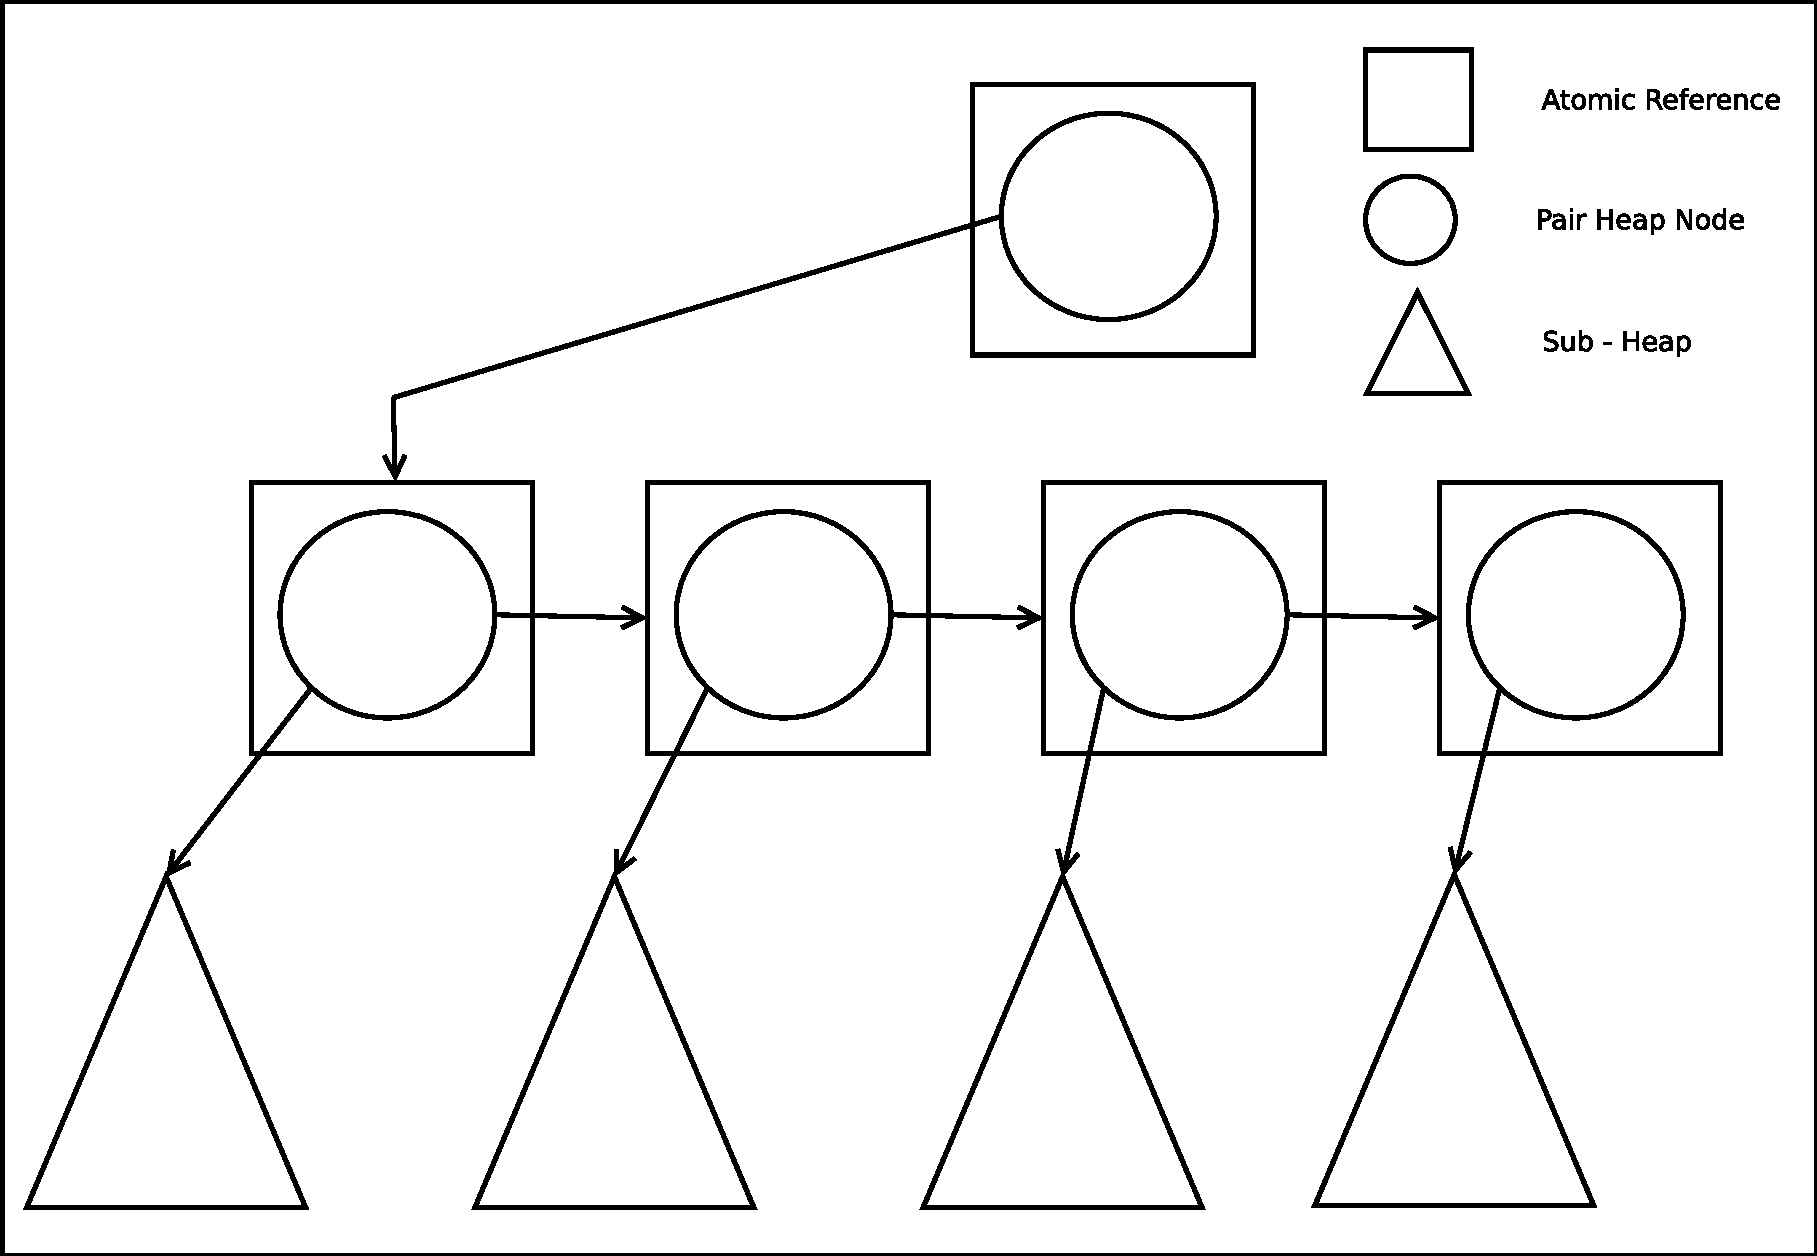
\includegraphics[width=0.5\textwidth]{img/PairHeapConcurrent-crop.pdf}
  \caption{Illustration of the concurrent pair heap structure. Pair heap nodes exist inside atomic references and hold atomic references to other heap nodes.}
  \label{fig:pairheap:structure}
\end{figure}


\subsection{Future Operators}
We briefly discuss the form of a parallelized \texttt{deleteMin} operator on Pairing heaps.
\texttt{deleteMin} follows what is essentially a Map-Reduce pattern: pairs of heaps are constructed
and then merged together to form a resultant heap. The first step has no contention between pairs
and is trivial to parallelize. Our \texttt{meld} operator can be used to merge heaps in parallel.

\section{Experimental Results}
Efficiency of the lock-free pairing heap will be examined by comparing the relative performance of Dijkstra's algorithm, backed by different heap structures, on large network data sets. Currently, we
plan to test three variants of Dijkstra's algorithm. The first variant will backed by a normal Skipqueue that performs a \texttt{decreaseKey} by removing the target node and readding it with a decreased key value.
The second variant will be backed with a Skipqueue that uses our optimized \texttt{decreaseKey} operator. The third variant will be backed with our lock-free pairing heap. We
will use real world data sets collected from the Stanford Large Network Dataset Collection \cite{slndc} and Harvard's Human Interactome Database \cite{hid}. We will additionally use two
synthetic graphs: a randomly generated dense graph and a randomly generated sparse graph.

%As pairing heaps are designed for efficiency in network applications such as shortest path finding, this is an ideal test case for this datastructure. Efficiency of parallel functionality will be examined for the data structure by determining runtime decrease by adding parallel functionality to the Dijkstra's implementation, through the use of the concurrent pairing heap.

\section{Real-world performance of Lock-Free Pairing Heaps and Skipqueues}
In non-lock-free Pairing heaps, nodes are inserted (a similar procedure is used for \texttt{decreaseKey})
into the heap by either replacing the root of the heap or inserting itself as a subheap to the root. It is clear to see that
parallel variants that preserve the general form of insertion operations will place un-due contention at the
root of the data structure. This is the main issue we foresee with our lock-free pairing heap: always inserting at the root
is a performance bottle-neck. Skipqueues, on the other hand, can insert elements in, e.g., the middle of the list in a less-contended way.

However, insertions into a Pairing heap run in asymptotically less time than a comparable Skipqueue insertion: a Pairing heap
insertion runs close to $\mathbb{O}(1)$ time but a Skipqueue insertion runs in $\mathbb{O}(\log n)$ time. This is due
to the differing methods used to balance the heap structure.


%\section{Lock-free Pairing Heaps}
%This section outlines our current thoughts about
%implementing a lock-free pairing heap.
%Lock-free procedures for pairing heaps will be implemented in a simlar manner to lock-free skip lists. The operat%ion delete min will require in depth analysis to avoid lock usage, as this method re-orders the entire heap. Other operations on the heap must remain active while a delete min operation is completing. A possible solution to this problem is to slightly loosen the restrictions on the heap properties. The loss of exactly following the pairing heap specification may lead to a lock-free solution while hopefully not compromising the integrity of the data structure.

%In
%\cite{shavit00} Shavit and Lotan construct
%a concurrent priority queue, coined a SkipQueue,
%based on Pugh's SkipList
%\cite{pugh90} data structure. We
%would like to adapt the principles outlined
%in \cite{fredman86} to Shavit SkipQueue.
%Specifically, we want to develop a corresponding
%\texttt{decreaseKey} operation on SkipQueues
%that allows an item in the heap to be
%decremented without the overhead of removing
%the item and adding a new item containing
%its decremented
%value.

%\section{Project Overview}

%This project will involve the following software
%development tasks:

%\begin{enumerate}
%  \item Develop a lock-based implementation of a pairing heap
%  \item Develop an implementation of Pugh's SkipLists
%  \item Develop an implementation of Shavit's SkipQueue.
%\end{enumerate}

%This project will involve the following research tasks:

%\begin{enumerate}
%  \item Propose an efficient \texttt{decreaseMin} operator for SkipQueues.
%  \item Determine if any additional optimizations can be made to enhance SkipQueues' performance
%    on the single-source shortest path problem.
%\end{enumerate}

%We will empirically evaluate the performance of a
%lock-based pairing heap, Shavit's SkipQueue, and
%our modified SkipQueue on a heap-backed version of Dijkstra's algorithm.
%We will test the performance of all these algorithms
%against the graph below with a varying number of threads.
%If we use C++ to implement lock-free pairing heaps we will use of the C++ pthreads library, as well as templates, to allow for the construction of a concurrent STL-like container class in C++. Further work may be explored by using the me%ssage passing interface (MPI).

%\begin{enumerate}
%\item A randomly-generated dense graph.
%\item A randomly-generated sparse graph.
%\item Graphs from Stanford's Large Network Dataset Collection \cite{slndc}
%\item Graphs from Harvard's Human Interactome Database \cite{hid}
%\end{enumerate}


% References
\bibliographystyle{abbrv}
\bibliography{proposal}

\end{document}
